\usepackage[utf8]{inputenc}
\usepackage[T1]{fontenc}\chapter{Realizácia riešenia}\label{chap:research}

Kapitola opísuje priebeh realizácie riešenia. Postup sa vo veľkej miere držal návrhu, avšak počas vývoja došlo k malým doplnkom. Na prácu s výpočtovo zložitými operáciami sme mali k dispozícii školský server, ktorý má dve grafické karty NVIDIA GeForce RTX 3060, každá 12 GB pamäte, CPU AMD Ryzen 9 5900X a 64 GB RAM. Na prihlásenie a vykonávanie príkazov na vzdialenom počítači bol použitý štandardný sieťový protokol. Prístup k serveru je zdieľaný medzi úzkou skupinou ľudí, preto pri jeho používaní trebalo brať ohľad aj na druhých používateľov.

\section{Experimentálne meranie}

Pred začiatkom merania sme sa oboznámili s odporúčaniami uvedenými v používateľskej príručke a vyskúšali testovaciu nahrávku. Kamera disponuje širokým záberom s rozlíšením 1920x1080. Na sledovanie pohybu šošoviek sú pripravené štyri kamery a ďalších šestnásť osvetľovačov. Všetko je integrované priamo v sklách okuliarov. Okuliare nijakým spôsobom nebránili vo výhľade a ich nosenie bolo veľmi prirodzené. Majú jemne zatienené sklá, pretože meranie je veľmi citlivé na priame osvetlenie.

% todo z okolia fakulty?
Počas jedného týždňa sa na meraní zúčastnilo osem ľudí. Všetci zúčastnení boli z okolia fakulty a jazdu absolvovali na svojom aute bez poskytnutia finančnej odmeny.Dvaja účastníci mali mierne poškodenie zraku do diaľky a počas jazdy nemali nasadené dioptrické okuliare a ani šošovky. Podľa ich subjektívneho názoru to jazdu nijak významne neovplyvnilo.

Jedna polovica účastníkov poznala celú trasu a druhá len určitú časť. V každom prípade bol vodič pred jazdou oboznámený, ktorou trasou pôjde a zároveň bol počas jazdy navigovaný spolujazdcom. Väčšia časť ľudí poznala čo je predmetom výskumu. V tabuľke \ref{table:1} sú uložené informácie k jednotlivým účastníkom.

V nahrávacom softvéry so po dokončení nahrávania zobrazila informácia o tom, pre akú percentuálnu časť záznamu boli zaznamenané pohľady. Nízke percento mohlo byť zapríčinené sveteľnými podmienkami a slabšou kalibráciou. Priemerná nameraná hodnota bola 63,6\%. Okuliare sú určené predovšetkým na interný priestor a pre vonkajší sa odporúča použiť nástavec na tienenie, ktorý sme nemali k dispozícii.

\begin{table}[ht]
\centering
\begin{tabular}{ |c c c c c|  }
\hline
meno & dioptrie & pozná cestu & pozná projekt & meranie \\
\hline
Dávid & - & áno & áno & 69\% \\
Matúš & 0.5 & časť & áno & 70\% \\
Viktor & 0.5 & časť & áno & 63\% \\
Zuzana & - & áno & áno & 33\% \\
Lukáš & - & časť & nie & 72\% \\
Jaroslav & - & áno & nie & 69\% \\
Zdenka & - & áno & nie & 45\% \\
Zuzana & - & časť & áno & 88\% \\
\hline
\end{tabular}
\caption{Informácie o účastníkoch experimentálneho merania.}
\label{table:1}
\end{table}

\section{Tobii Pro Lab}

Spoločnosť Tobii okrem hardvéru dodáva aj softvér na analýzu záznamu, čím ponúka kompletné riešenie pre výskum. Tobii Pro Lab poskytuje grafické používateľské rozhranie a špeciálne softvérové funkcie, ktoré pomáhajú s analýzou pohľadov. V zásade podporuje dva spôsoby, podľa ktorých sa dajú získať analytické údaje. 

Prvým spôsobom je označenie oblasti, na ktorom sa nachádza objekt záujmu. Ku zvýšeniu efektivity má pomôcť automatické označovanie oblastí, kde stačí označiť objekt na prvej a na poslednej snímke, na ktorej bol viditeľný. Na základe tejto informácie a predpokladaným pohybom objektu, softvér vypočíta oblasť pre všetky zvyšné snímky v sekvencii. Bohužiaľ v našej práci sa to neukázalo ako dobré riešenie, pretože pohyb reklamy v nahrávkach nebol jednoduchý. Takmer na žiadnej snímke medzi začiatkom a koncom nebola oblasť reklamy označená správne. 

Druhou možnosťou je priložiť do softvéru referenčný obrázok, na ktorom je sledovaný objekt. Potom ako sa vyberie časový interval, v ktorom sa očakáva výskyt sledovaného objektu, softvér automatický získa výstup toho, na ktorú časť objektu sa človek pozeral. Toto riešenie takisto zlyhalo, nakoľko softvér ani po viacerých pokusoch nedokázal priradiť k obrázku žiadne pohľady.
\\
\begin{figure}[ht]
    \centering
    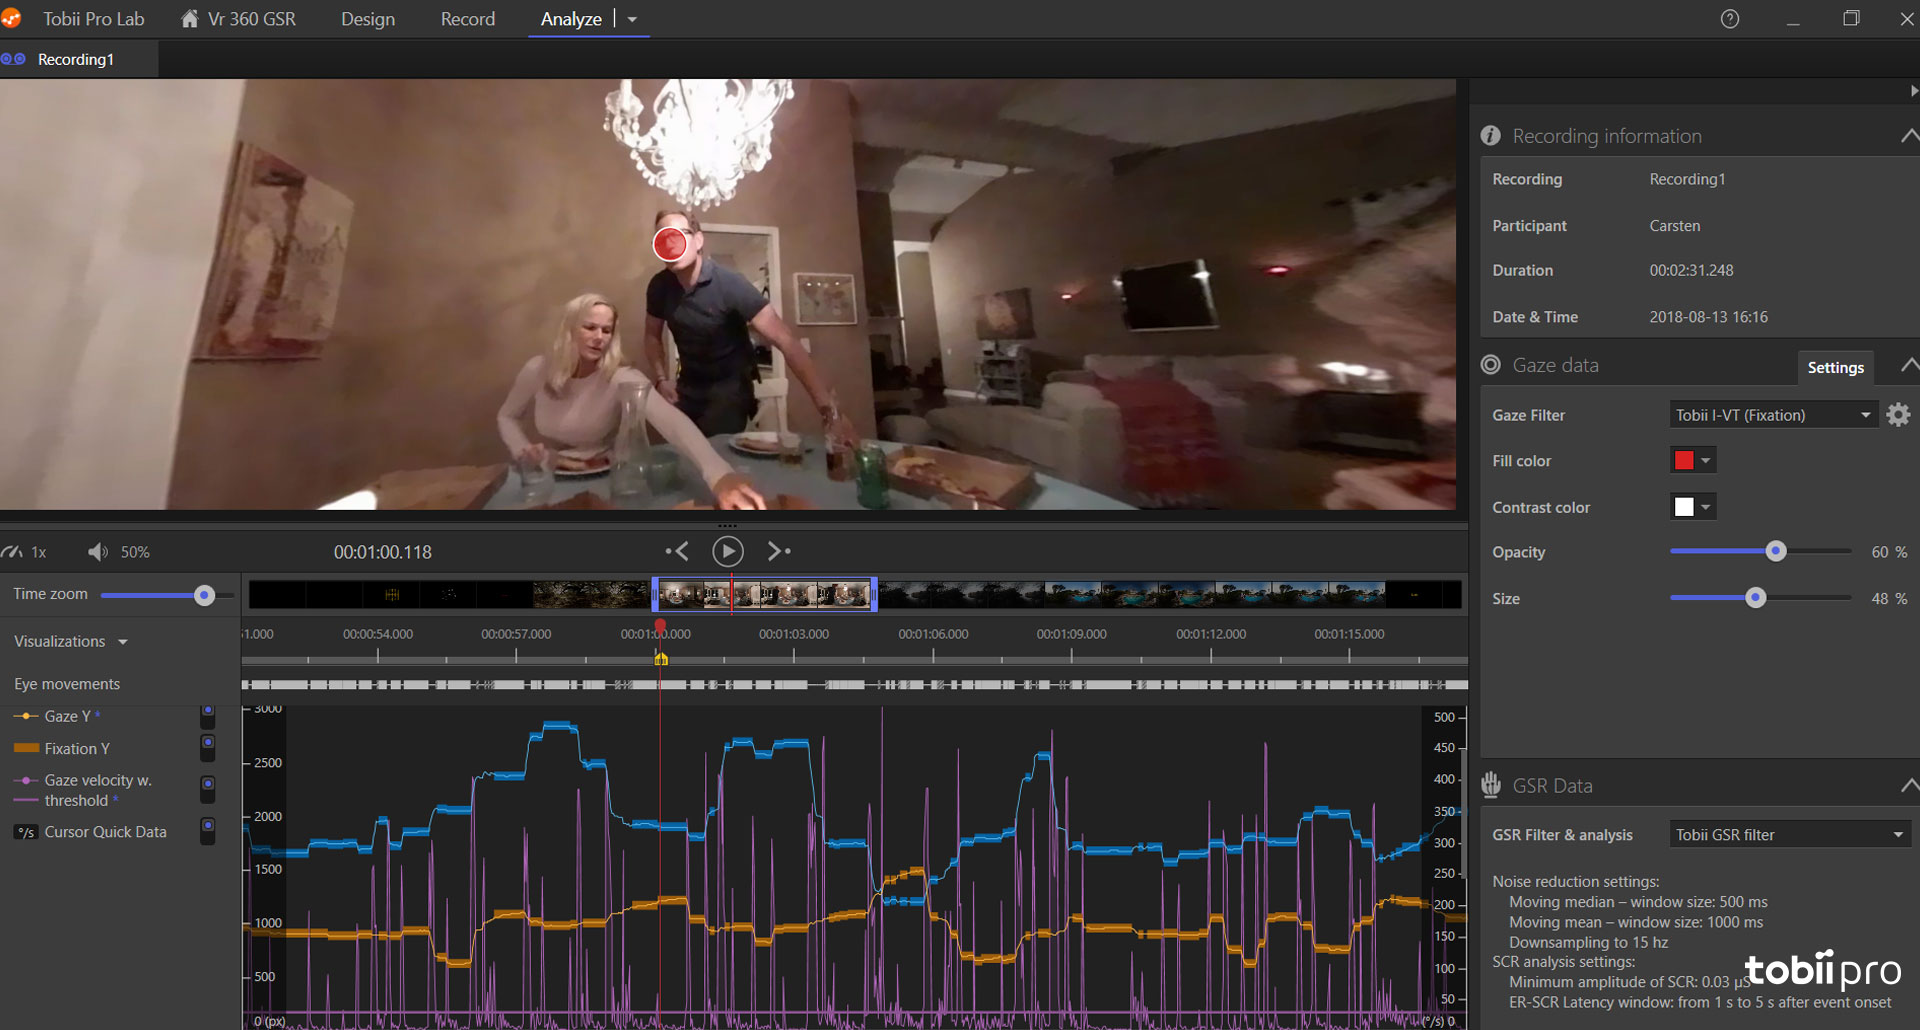
\includegraphics[width=1\textwidth]{images/02/tobiiprolab3.jpg}
    \caption{TODO, nahradiť obrázkom, kde je zle vypočítaná oblasť pre reklamu ... nemám :(}
    \label{img:lab}
\end{figure}

% tensorboard https://medium.com/mlearning-ai/remote-tensorboard-viewing-on-your-local-browser-b0dc5c5a634a     and     https://pytorch.org/docs/stable/tensorboard.html

\section{Detektor reklám}

Narozdiel od predchádzajúcich YOLO verzií sa dá YOLOv8 nainštalovať a importovať do projektu priamo ako knižnica pre Python. Spolu s ňou sa do prostredia nainštalujú ďalšie dôležité knižnice ako matplotlib, opencv-python, scipy, torch, torchvision a iné. Trénovanie sa spúšťa pomocou jedného príkazu, kde argumenty špecifikujú hodnoty pre parametre.

Potrebné je nastaviť tri parametre:

\begin{enumerate}
    \item zdroj dát,  v našom prípade priečinok uložený na disku, ale ako zdroj sa dá použiť aj živý záznam z kamery alebo odkaz na video zverejnené na internete
    \item počiatočné váhy,  dajú sa stiahnuť z oficiálnej dokumentácie pre YOLOv8. Na výber je 5 modelov, ktoré sa líšia počtom parametrov, rýchlosťou a presnosťou
    \item počet epoch, vo väčšine prípadov, sme zvolili 128 epoch, vzhľadom na to, že jeden cyklus trval približne 10 minút
\end{enumerate}

Ostatné parametre pre tréning majú hodnoty prednastavené podľa všeobecného odporúčania pre prvý tréning. Okrem 

\subsubsection{Dataset}

Väčšina obrázkov v Mapillary Vistat je vyohtovených z vnútra auta, prípadne zo strechy. Obrázky zachytávajú premávku vo vnútri mesta, kde sa nachádza veľa budov, chodníkov, dopravných značení a mnoho iných objektov z cestnej premávky vrátene reklamných plôch.

Anotácie sú uložené vo formáte, ktorý nie je kompatibilný s formátom pre YOLO. Počas úpravy formátu sme zároveň vynechali obrázky, ktoré neobsahovali reklamu, čím sa počet obrázkov znížil na približne 20000 obrázkov. Pri prvom tréningu sme si všimli, že veľká chybovosť nastáva práve pri najmenšie označených reklamách. Najmenšie reklamy boli označené v takej diaľke, že by sa nedalo s istotou povedať, či sa vodič skutočne pozeral na reklamu, alebo na iný objekt. Preto sme z pôvodných dát vytvorili druhú verziu, kde sme ponechali len také obrázky, kde reklamná plocha tvorí aspoň 0,1\% z obrázka. Takouto úpravou mala druhá verzia dát takmer o polovicu menej obrázkov.

Pripravili sme ešte tretiu verziu dát, kde sme k vytriedeným dátam pridali 350 nových obrázkov s anotáciami reklám. Obrázky pochádzali z videí nahratých cez eyetracker, ktoré boli mimo meranú trasu. Všetky tri verzie dát sme rozdelili na tréningovú, validačnú a testovaciu sadu, v pomere 8:1:1.

\section{Sledovanie reklám}

Na sledovanie reklám vo videách sa nám podarilo nájsť repozitár, v ktorom je možné vyskúšať viaceré sledovacie metódy. V čase keď sme s ním pracovali, podporoval metódy OC-SORT \cite{ocsort}, Deep OC-SORT \cite{TODO}, StrongSORT \cite{strongsort}, BoTSORT \cite{TODO} a ByteTrack \cite{bytetrack}. Všetky metódy sú implementované v jazyku Python a využívajú knižnicu PyTorch. Vychádzajú z metódy SORT (Simple Online and Realtime Tracking), ktorá na sledovanie objektov používa Kalmanov filter a Hungarian algoritmus \cite{sort}.

Vstupné video sa spracováva postupne po jednej snímke. Zo snímky sa pomocou modelu získajú detekcie, ktorým sa podľa asociácie priradí referencie. Naraz sa dajú sa sledovať viaceré objety a triedy. Výstupom sledovacej metódy sú detekcie s priradenou referenciou \ref{img:tracking}.

 \begin{figure}[ht]
     \centering
     
\includegraphics[width=1\textwidth]{images/02/placeholder.png}
     \caption{Postup pri sledovaní objekov vo videu.}
     \label{img:tracking}
 \end{figure}

Každá metóda má konfiguračný súbor, kde sa dá nastaviť viacero parametrov, ktoré ovplyvňujú sledovanie objektu. Dva najdôležitejšie parametre sú prahová hodnota pre detekciu objektu a prahová hodnota pre asociáciu k objektom v predchádzajúcich snímkach. Okrem toho sa dá nastaviť počet predchádzajúcich snímok, v ktorých sa porovnáva asociácia objektov, minimálny počet snímok na vytvorenie sekvencie a niekoľko ďalších špecifických pre jednotlivé metódy. Napríklad pre StrongSort maximálna vzdialenosť lokalizácie a pre OC-SORT výber asociačnej funkcie.

\subsection{Pomocné dáta a model}

Na priblíženie sa ku skutočným výskytom reklám v nahrávkach, sme sa rozhodli natrénovať nový pomocný model. Pre tento účel sme pripravili dataset, ktorý bol vytvorený zo snímok vystrihnutých z nahrávok experimentu. Reklamné plochy na vystrihnutých snímkam sme najskôr dali detegovať pomocou najlepšieho modelu, ktorý sme v tom momente mali. Získané označenia sme spolu s obrázkami pridali do webovej aplikácie Darwin v7labs \cite{v7}, kde sme následne opravili vzniknuté chyby z detekcie. Opraviť bolo treba približne každý druhý obrázok, ktorých spolu bolo takmer tisíc.

Pomocný model dosahoval pri sledovaní výrazne viac detekcií. Pre účely dosiahnuť čo najviac snímok s reklamou, sme metódu StrongSort nastavili tak, aby mala čo najväčšiu citlivosť detekcie. Samozrejme sa tým znížila celková presnosť sledovania, ale to v podstate nebolo dôležité, pretože sme vedeli, že pred pokračovaním budeme potrebovať každú reklamu označiť rovnakou referenciou v každom videu, aby sme mohli analyzovať pohľady na reklamu v každom videu.

% Metódu s vysokou citlivosťou sme použili na detekciu reklám z každej nahrávky z merania.
Museli sme opraviť dve chyby, falošne pozitívne detekcie a nesprávne priradenie referencie. Prakticky to znamenalo, že sme vytvorili kópie nahrávok, v ktorej boli vykreslené všetky detekcie s uvedenou referenciou. Pokiaľ išlo o správnu detekciu reklamy, tak sme priradenú referenciu nahradili poradovým číslom danej reklamy, ktorá bola rovnaké pre každé video.

Dosiahli sme tým korekciu oboch chýb a získané označenia sme ďalej považovali za skutočne pravdivé údaje. Označenia sme zapísali do textového súboru vo formáte MOT pre každé video samostatne. Každá snímka, na ktorej sa nachádzala reklama bola zapísaná v samostatnom riadku s hodnotami pre poradie snímky, referenciu reklamy, x a y súradnice ľavého horného rohu a pre rozmery reklamy.

\section{Významnosť reklám}

Zo získaných informácií, na ktorých snímkach sa nachádza reklama, sme mohli začať analyzovať pohľady vodiča. V tomto bode sme zistili, že pohľady boli zaznamenané v počte 50 snímok za sekundu, kým video bolo nahrávané v počte 25 snímok za sekundu. To znamená, že pokiaľ bol pohľad zaznamenaný bez straty mali sme pre každú snímku z videa dva pohľady.

Kvôli nedokonalému nahrávaniu na niektorých snímkach chýbal jeden, alebo dokonca oba pohľady. Pokiaľ sme pre snímok zaznamenali chýbajúci pohľad, vypočítali sme jeho predikciu pomocou dvoch predchádzajúcich pohľadov. Pre výpadok pohľadu na viac ako dve snímky sme predikciu nepočítali a snímok sme z analýzy vynechali.

Pre každú snímku, na ktorej bola reklama a zaznamenaný pohľad, sme porovnali ich prienik. Získali sme tým informáciu o počte snímok, kde pohľad smeroval na reklamu. Počet snímok sme vynásobili dĺžkou trvania jednej snímky, čím sme získali časový údaj sledovanosti. Podľa dĺžky sledovanosti sme vyhodnotili významnosť reklamy pre každého vodiča samostatne a následne vypočítali konečnú významnosť pomocou mediánu.

 \begin{figure}[ht]
     \centering
     
\includegraphics[width=1\textwidth]{images/02/placeholder.png}
     \caption{Ukážka prieniku a neprieniku, obrázok a), b).}
     \label{img:tracking}
 \end{figure}

\section{Klasifikácia reklamy}

% can object tracking improve object detection?

% Yes, object tracking can improve object detection. Object tracking can be used to refine the object detection process by providing additional information about the location and movement of objects in a video stream. By tracking objects across multiple frames, object tracking algorithms can help to reduce false positives and false negatives in the object detection process. For example, if an object detection algorithm detects an object in one frame but fails to detect it in the next frame, an object tracking algorithm can use the object's previous position and movement to predict its location in the current frame. This can help to reduce the number of false negatives and improve the accuracy of the object detection algorithm. Additionally, object tracking can be used to filter out false positives in the object detection process. By tracking an object across multiple frames, an object tracking algorithm can verify that the object is indeed present and is not just a false positive detection. This can help to improve the precision of the object detection algorithm. Overall, object tracking and object detection are complementary techniques that can be used together to improve the accuracy and robustness of computer vision systems.